\chapter{Experiments and Benchmarking}
\label{chp:contrib_ResultsDiscussion}

\section{Modified Forward Dynamics Benchmark}

The introduction of motor dynamics in the context of a recursive forward dynamics algorithm like \ac{ABA}, involves additional computations that are not present in the original algorithm. In this section, we present a benchmark that compares the performance of the modified \ac{ABA} algorithm with the original one, in order to evaluate the impact of the additional computations on the performance of the algorithm. Furthermore, the accuracy of the modified \ac{ABA} algorithm is evaluated by comparing the results with the ones obtained with the modified Inertia-Matrix method.

Regarding the computational performance, the modified \ac{ABA} algorithm is expected to be slower than the original one, due to the additional computations required to compute the motor dynamics. However, from the results reported in ADD REF TO RESULTS, it is possible to see that the modified \ac{ABA} algorithm is comparably fast to the original one, with a difference of less than $1\%$ in the execution time. This is due to the fact that the additional computations required to compute the motor dynamics are negligible compared to the other computations required by the algorithm.

When evaluating the difference between the results obtained with the modified \ac{ABA} algorithm and the modified Inertia-Matrix method, it is possible to see that the difference depends on the motor inertia values. In particular, the difference is larger for the joints with a smaller motor inertia, while it is smaller for the joints with a larger motor inertia.



\section{Robot Codesign Results}

In this section, we present the results of the robot codesign process, which is the main contribution of this work. We start by presenting the results of the \ac{RL} framework, which is used to optimize the control strategy of the system. Then, we present the results of the \ac{RL} framework with the addition of the genetic algorithm.

\subsection{RL Framework}

For the reinforcement learning training, we opted for the use of \textit{Weights {\&} Biases}\footnote{\url{https://wandb.ai}}, a tool that allows for the tracking of the training metrics and the hyperparameters used during the training. In opposition to the most common \textit{Tensorboard}\footnote{\url{https://www.tensorflow.org/tensorboard}} tool, \textit{Weights {\&} Biases} supports online logging, which allows for the real-time monitoring of the training metrics and more extensive logging capabilities.


\subsubsection{Cartpole Swing-Up}

For the cartpole swing-up task, the metrics obtained during the training with \texttt{stable\_baselines3} together with \jaxsim are reported in \cref{fig:cartpoleresults}.

\begin{figure}
    \centering
    \caption{Cartpole RL Training Metrics}
    \label{fig:cartpoleresults}
    \subfloat[Explained Variance]{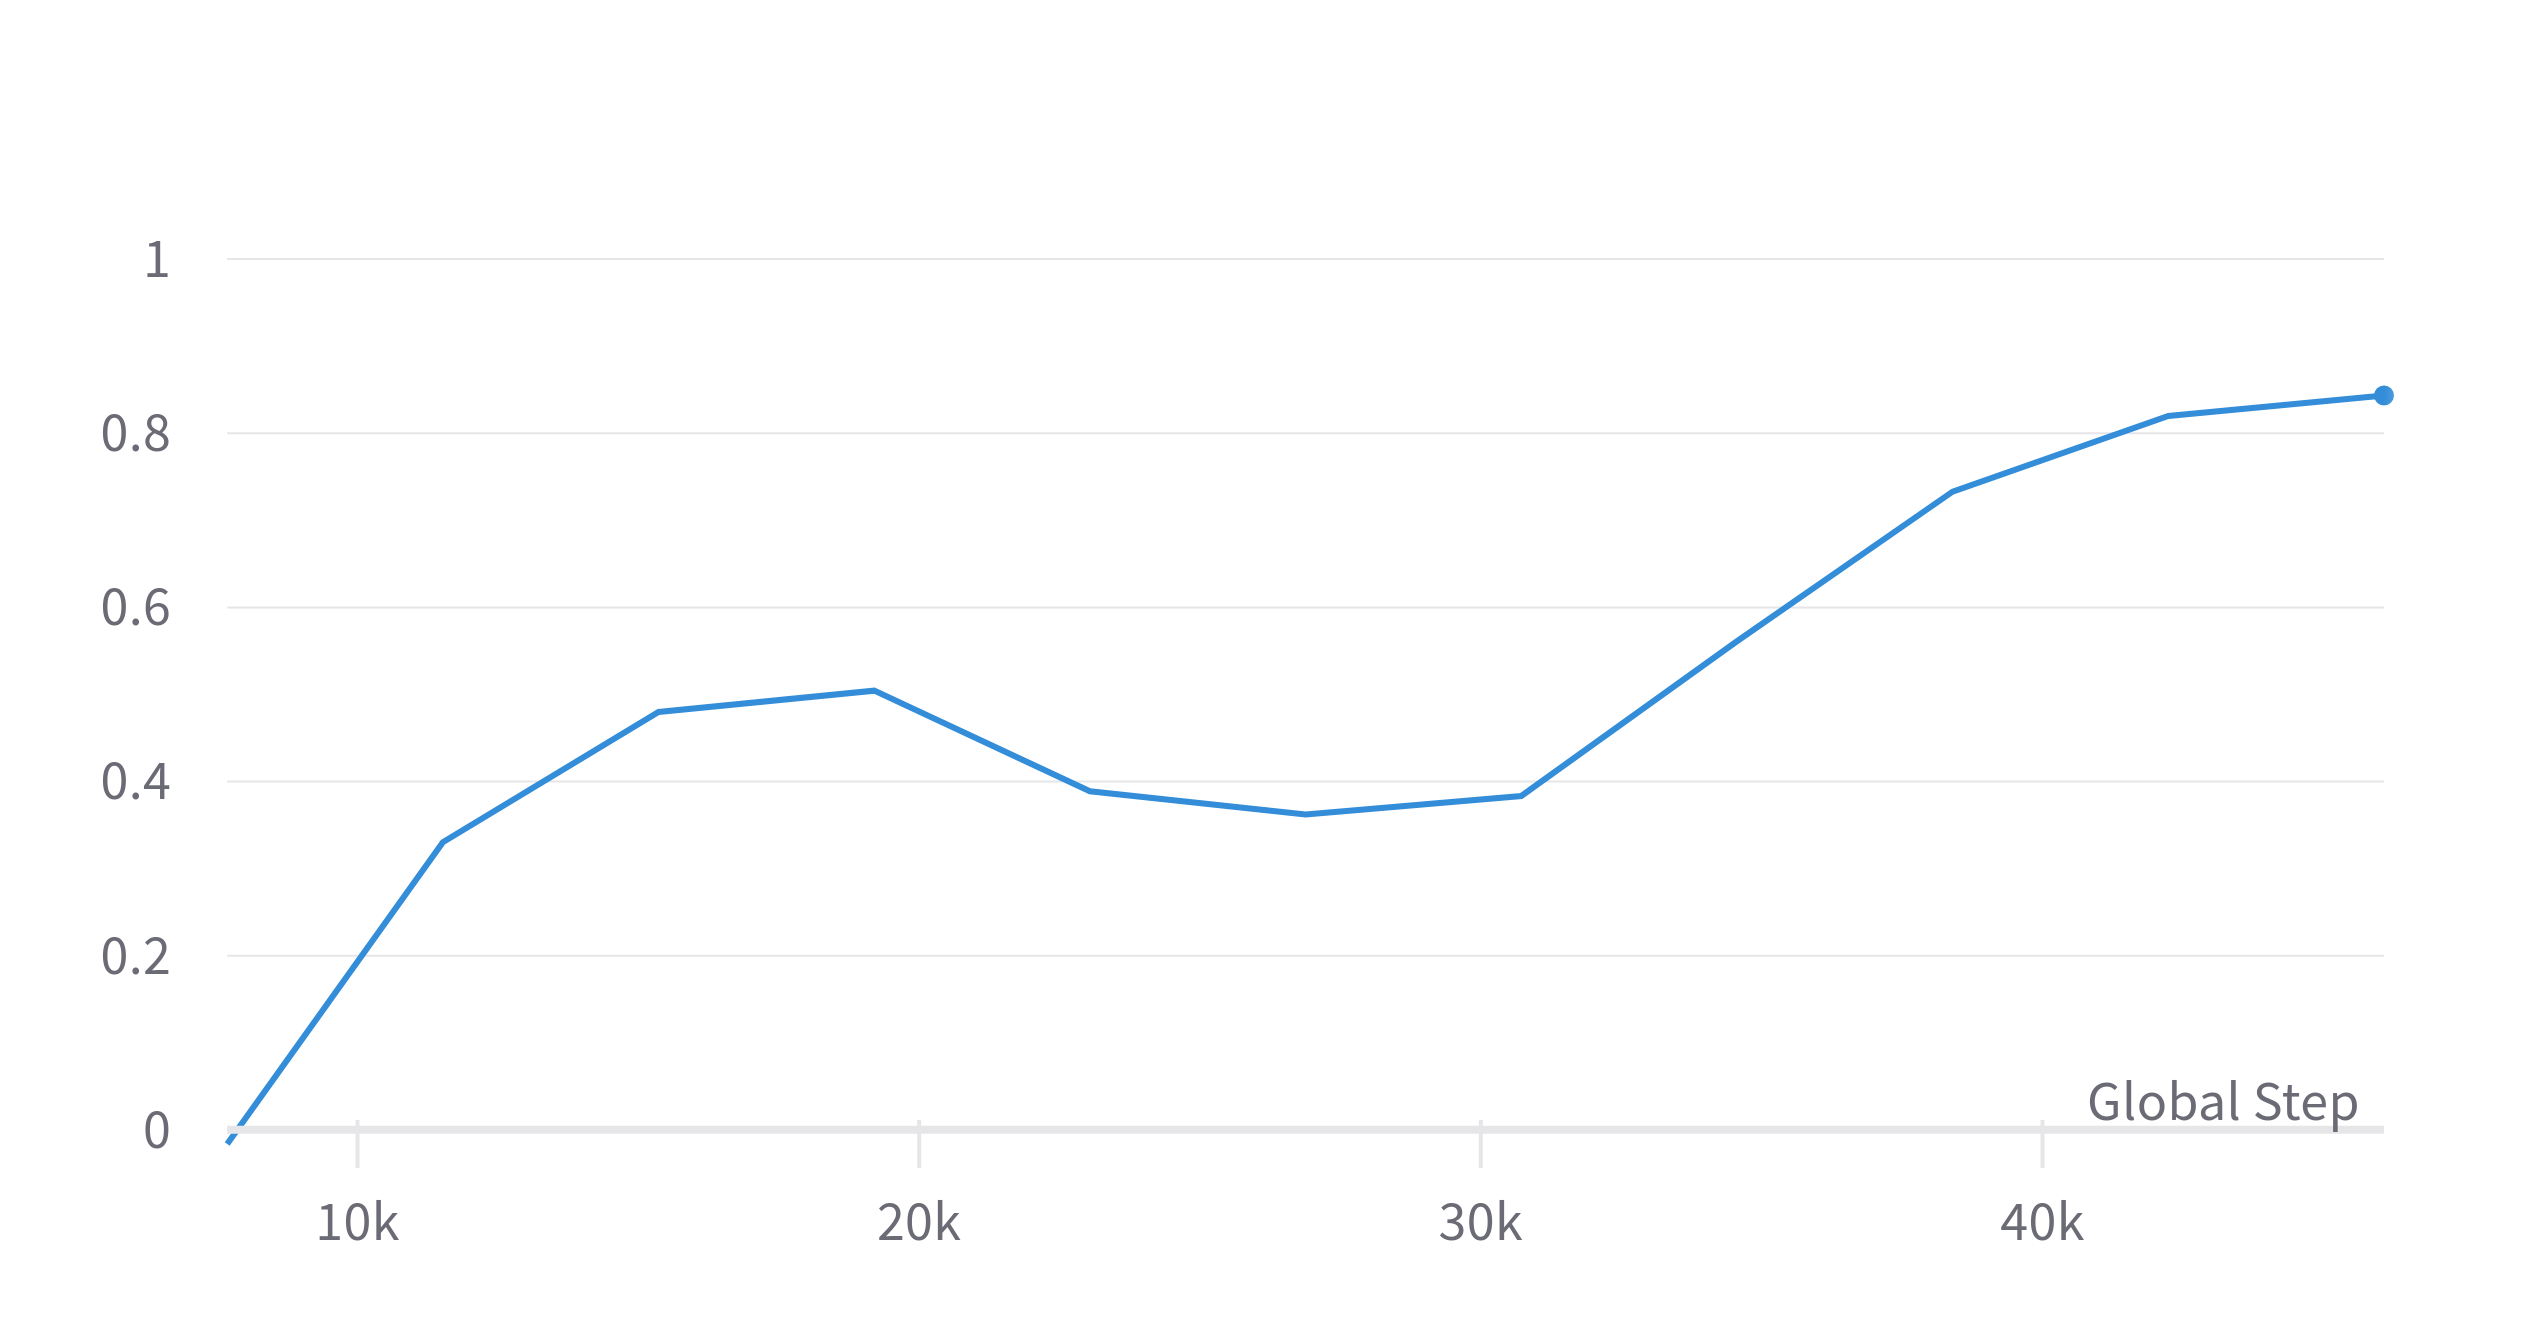
\includegraphics[width=0.45\textwidth]{Images/Results/expvariance_cartpole.png}}
    \subfloat[Approximated KL]{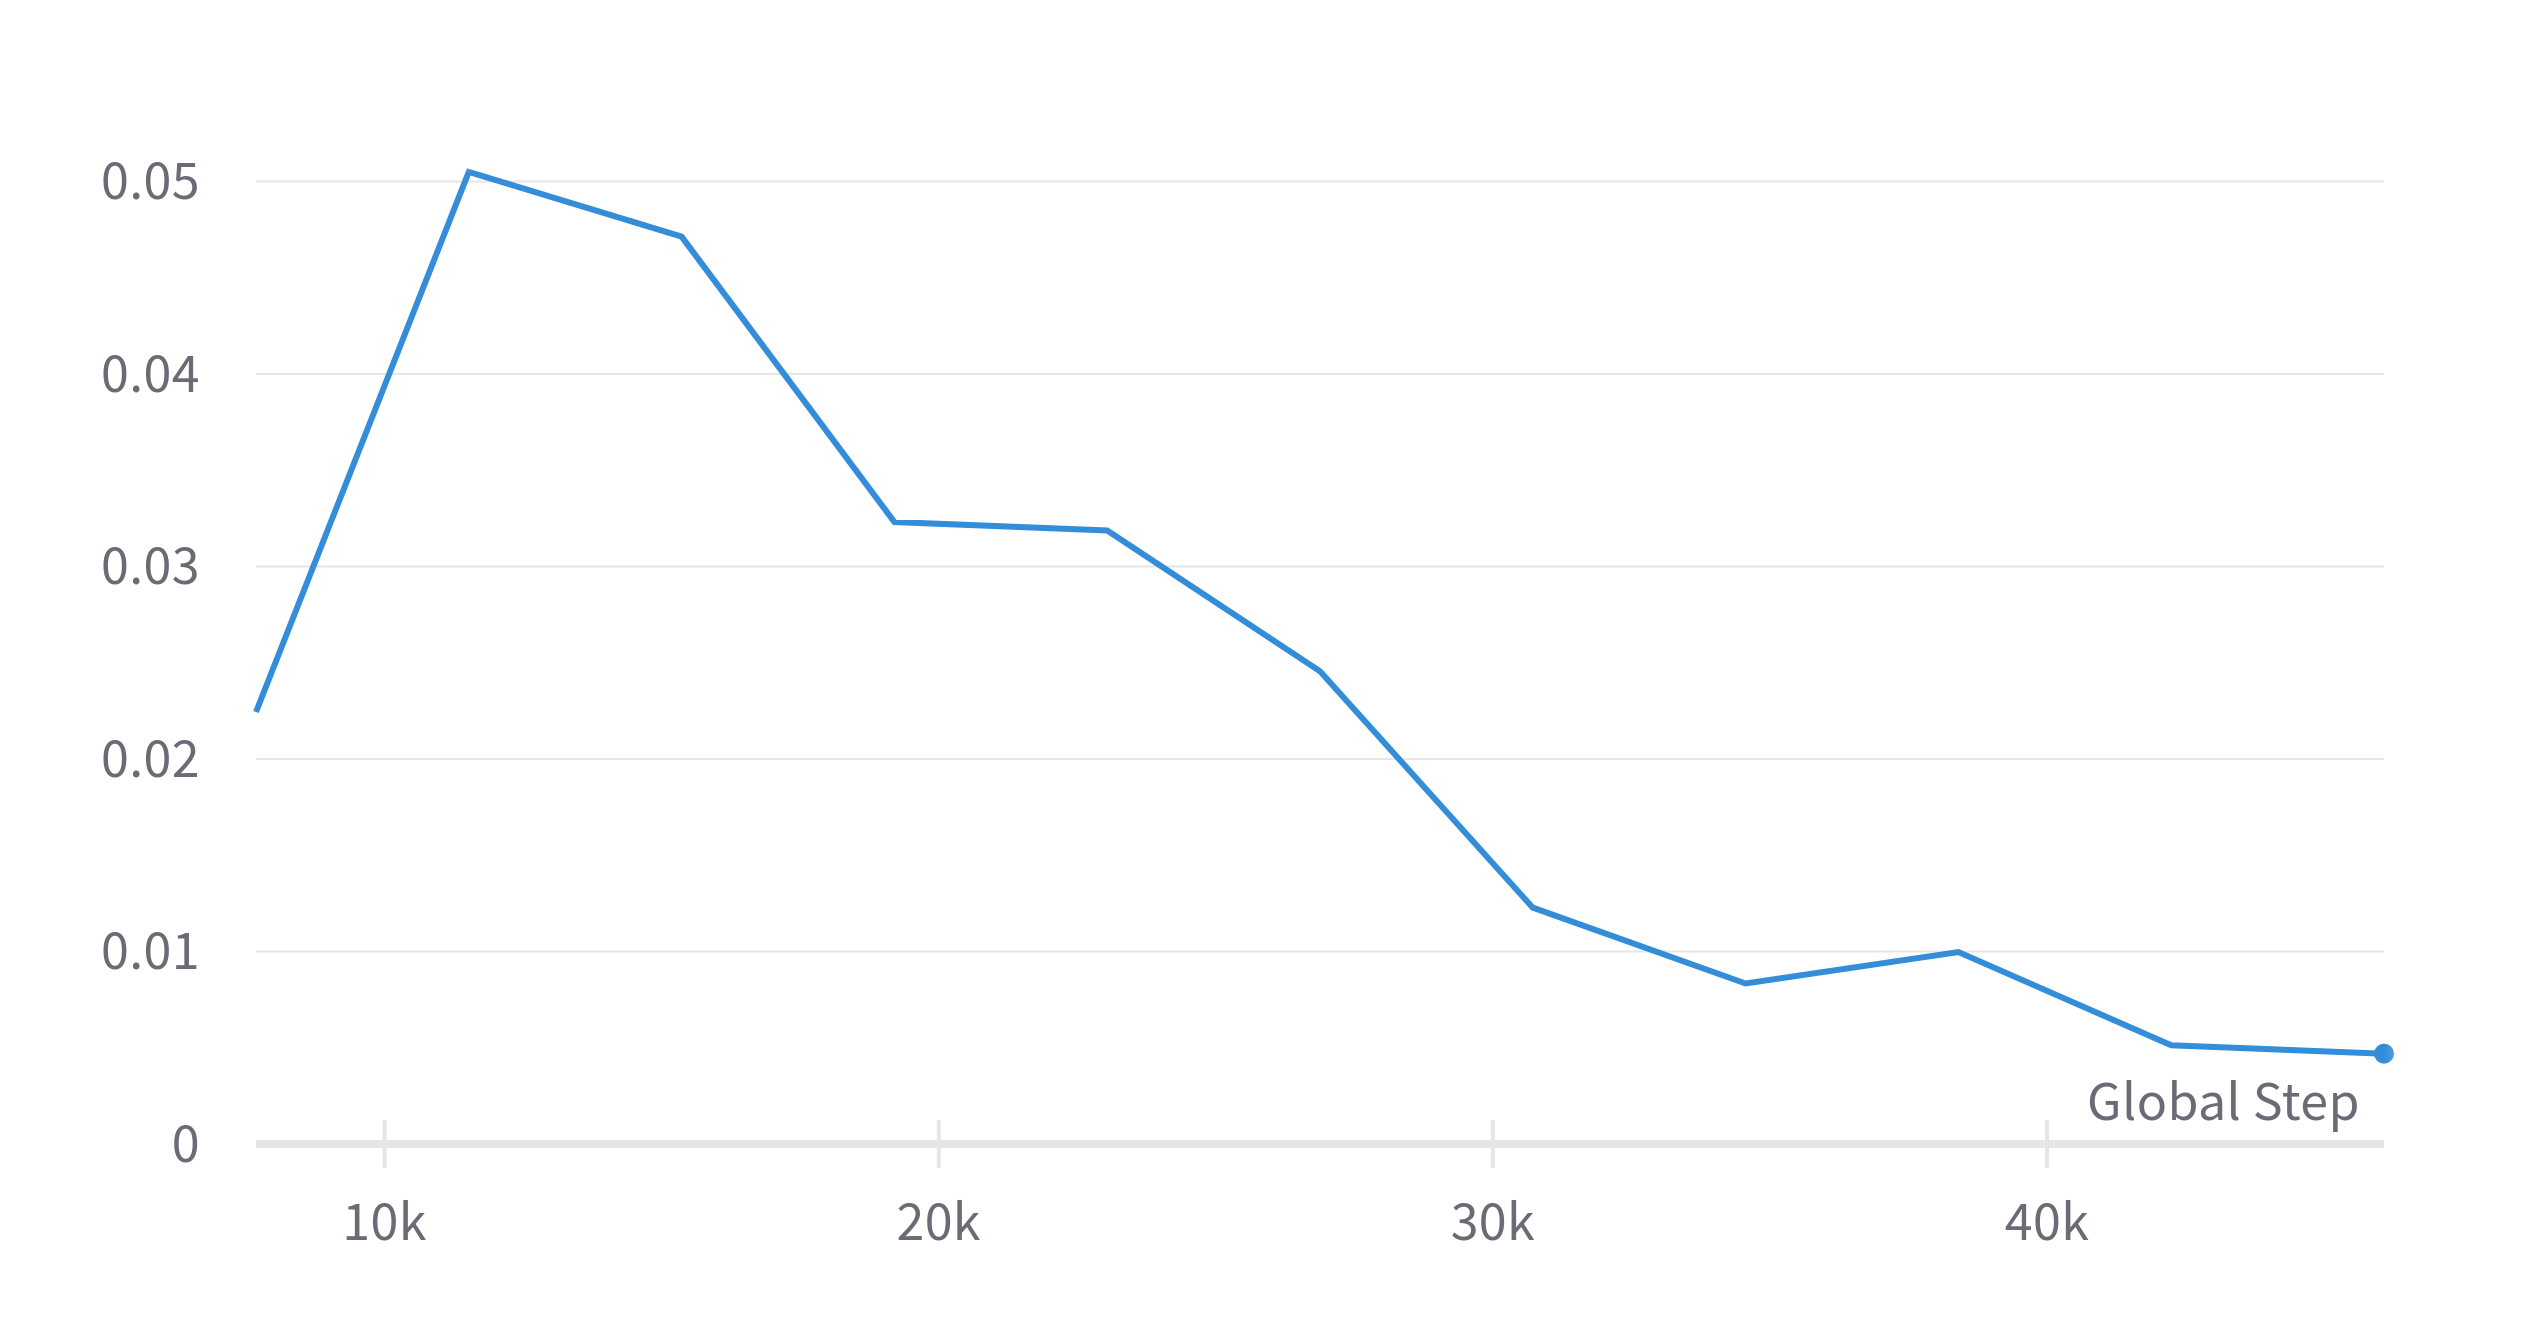
\includegraphics[width=0.45\textwidth]{Images/Results/kl_cartpole.png}} \\
    \subfloat[Value Loss]{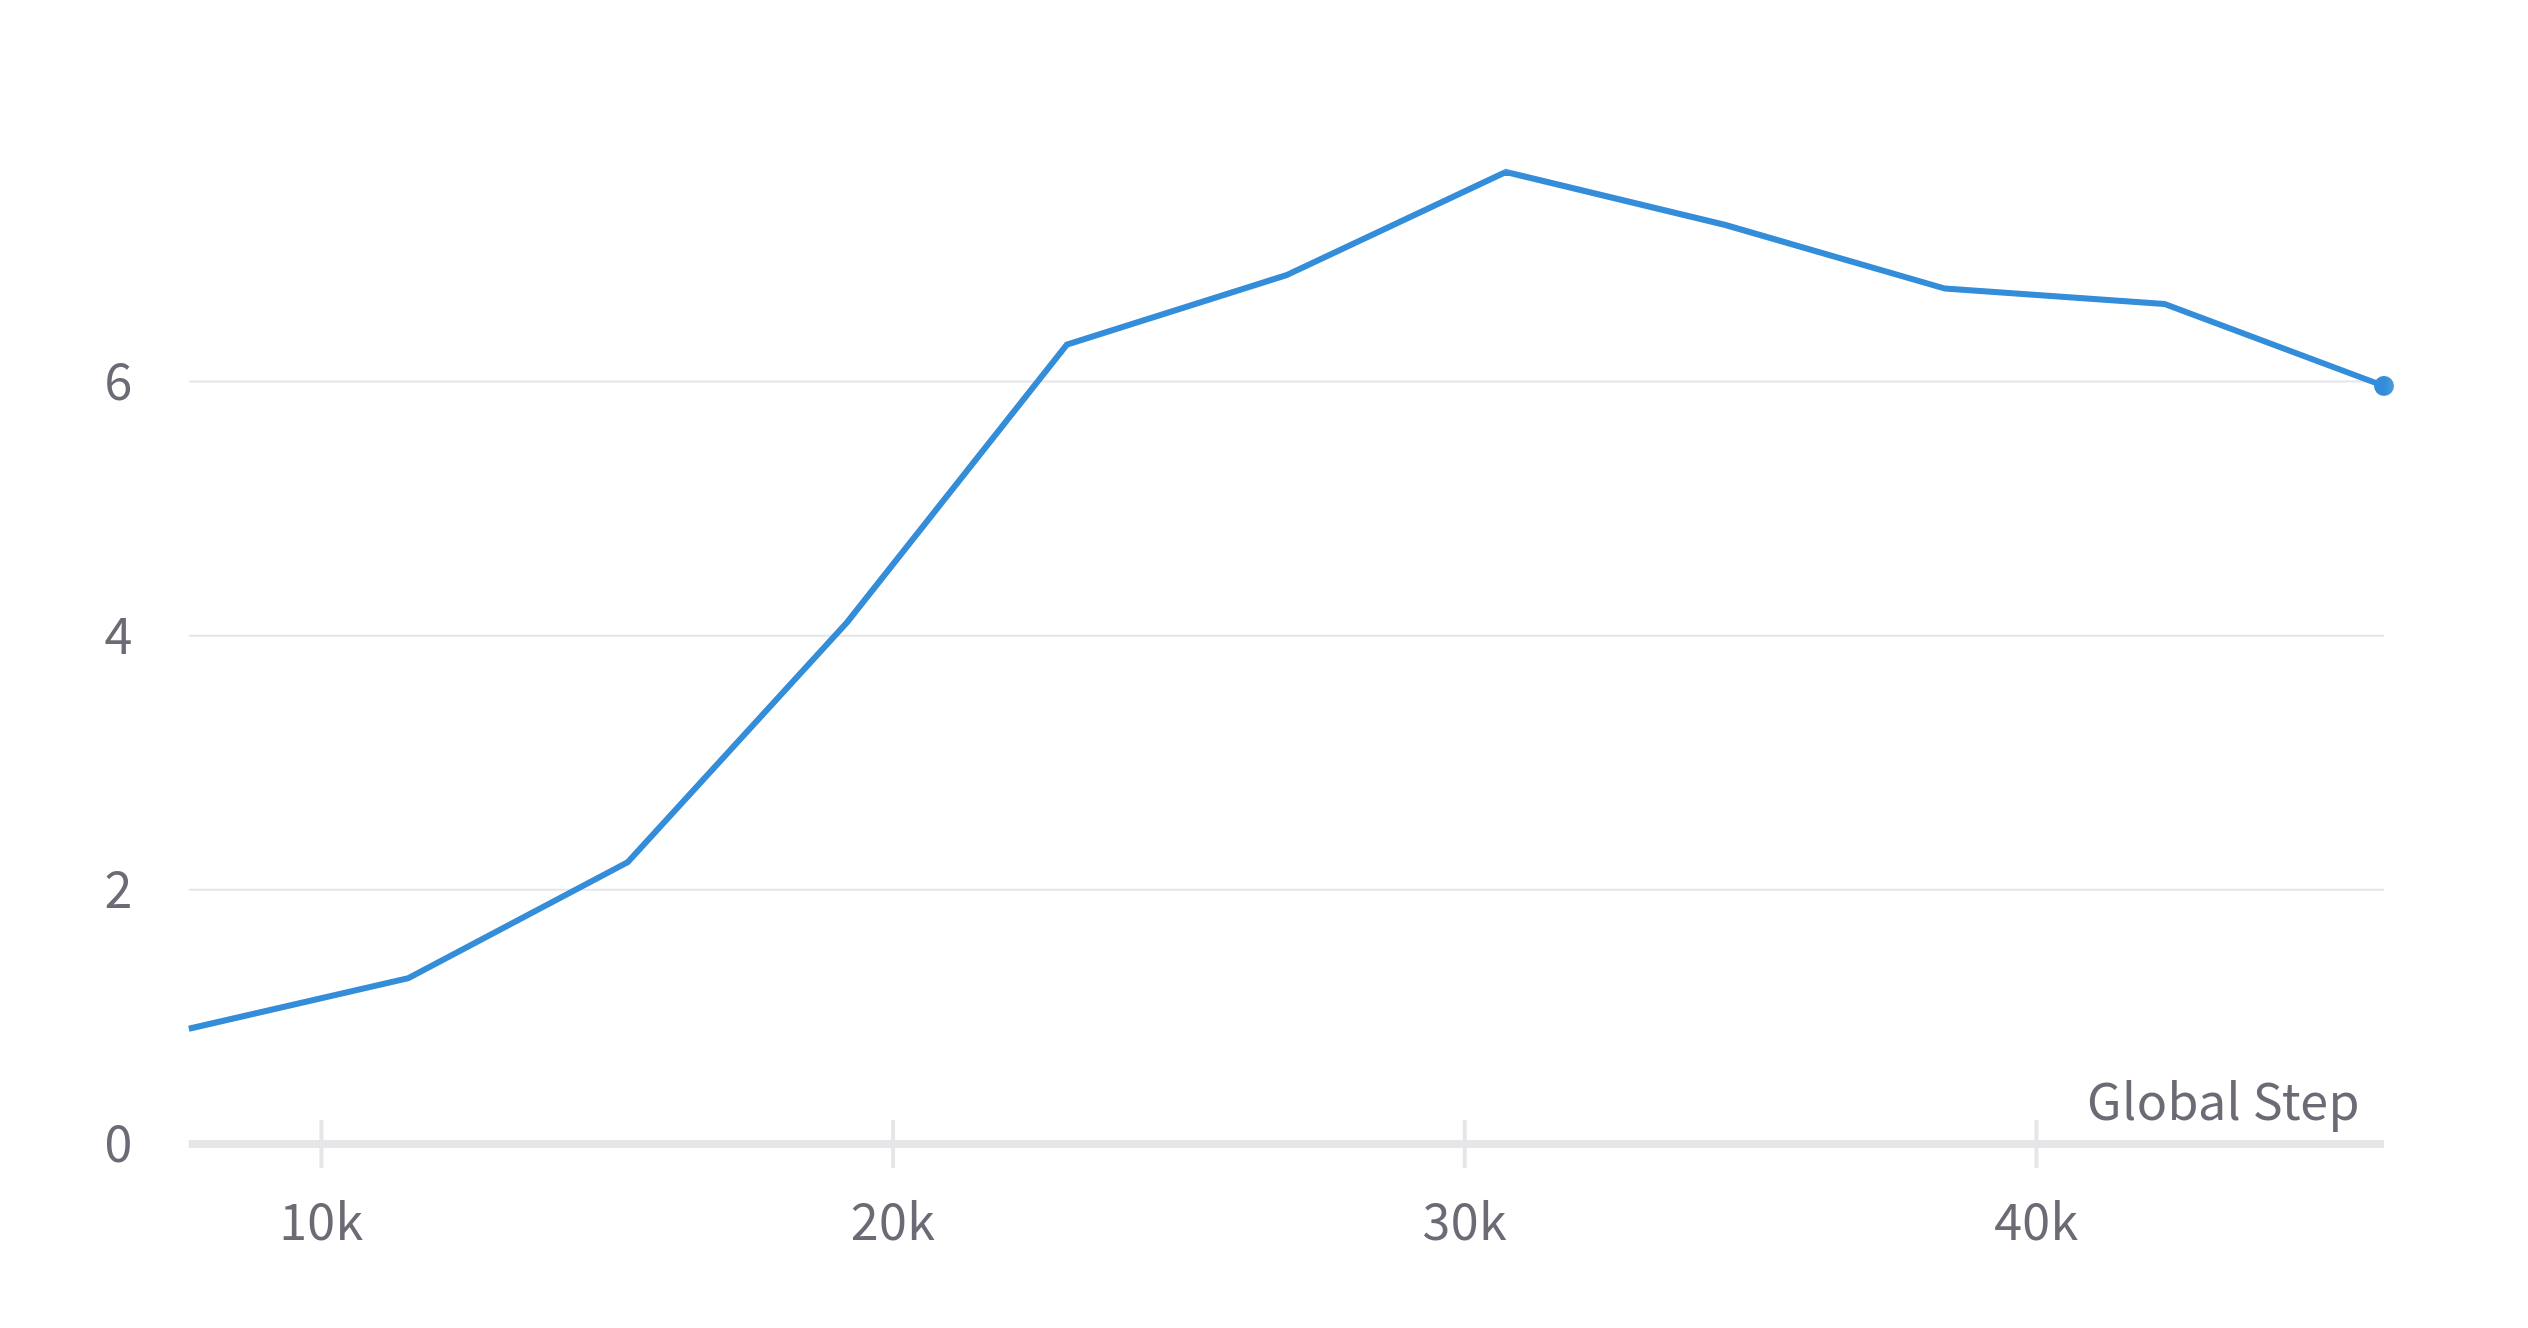
\includegraphics[width=0.45\textwidth]{Images/Results/loss_value_cartpole.png}}
    \subfloat[Rollout Metrics]{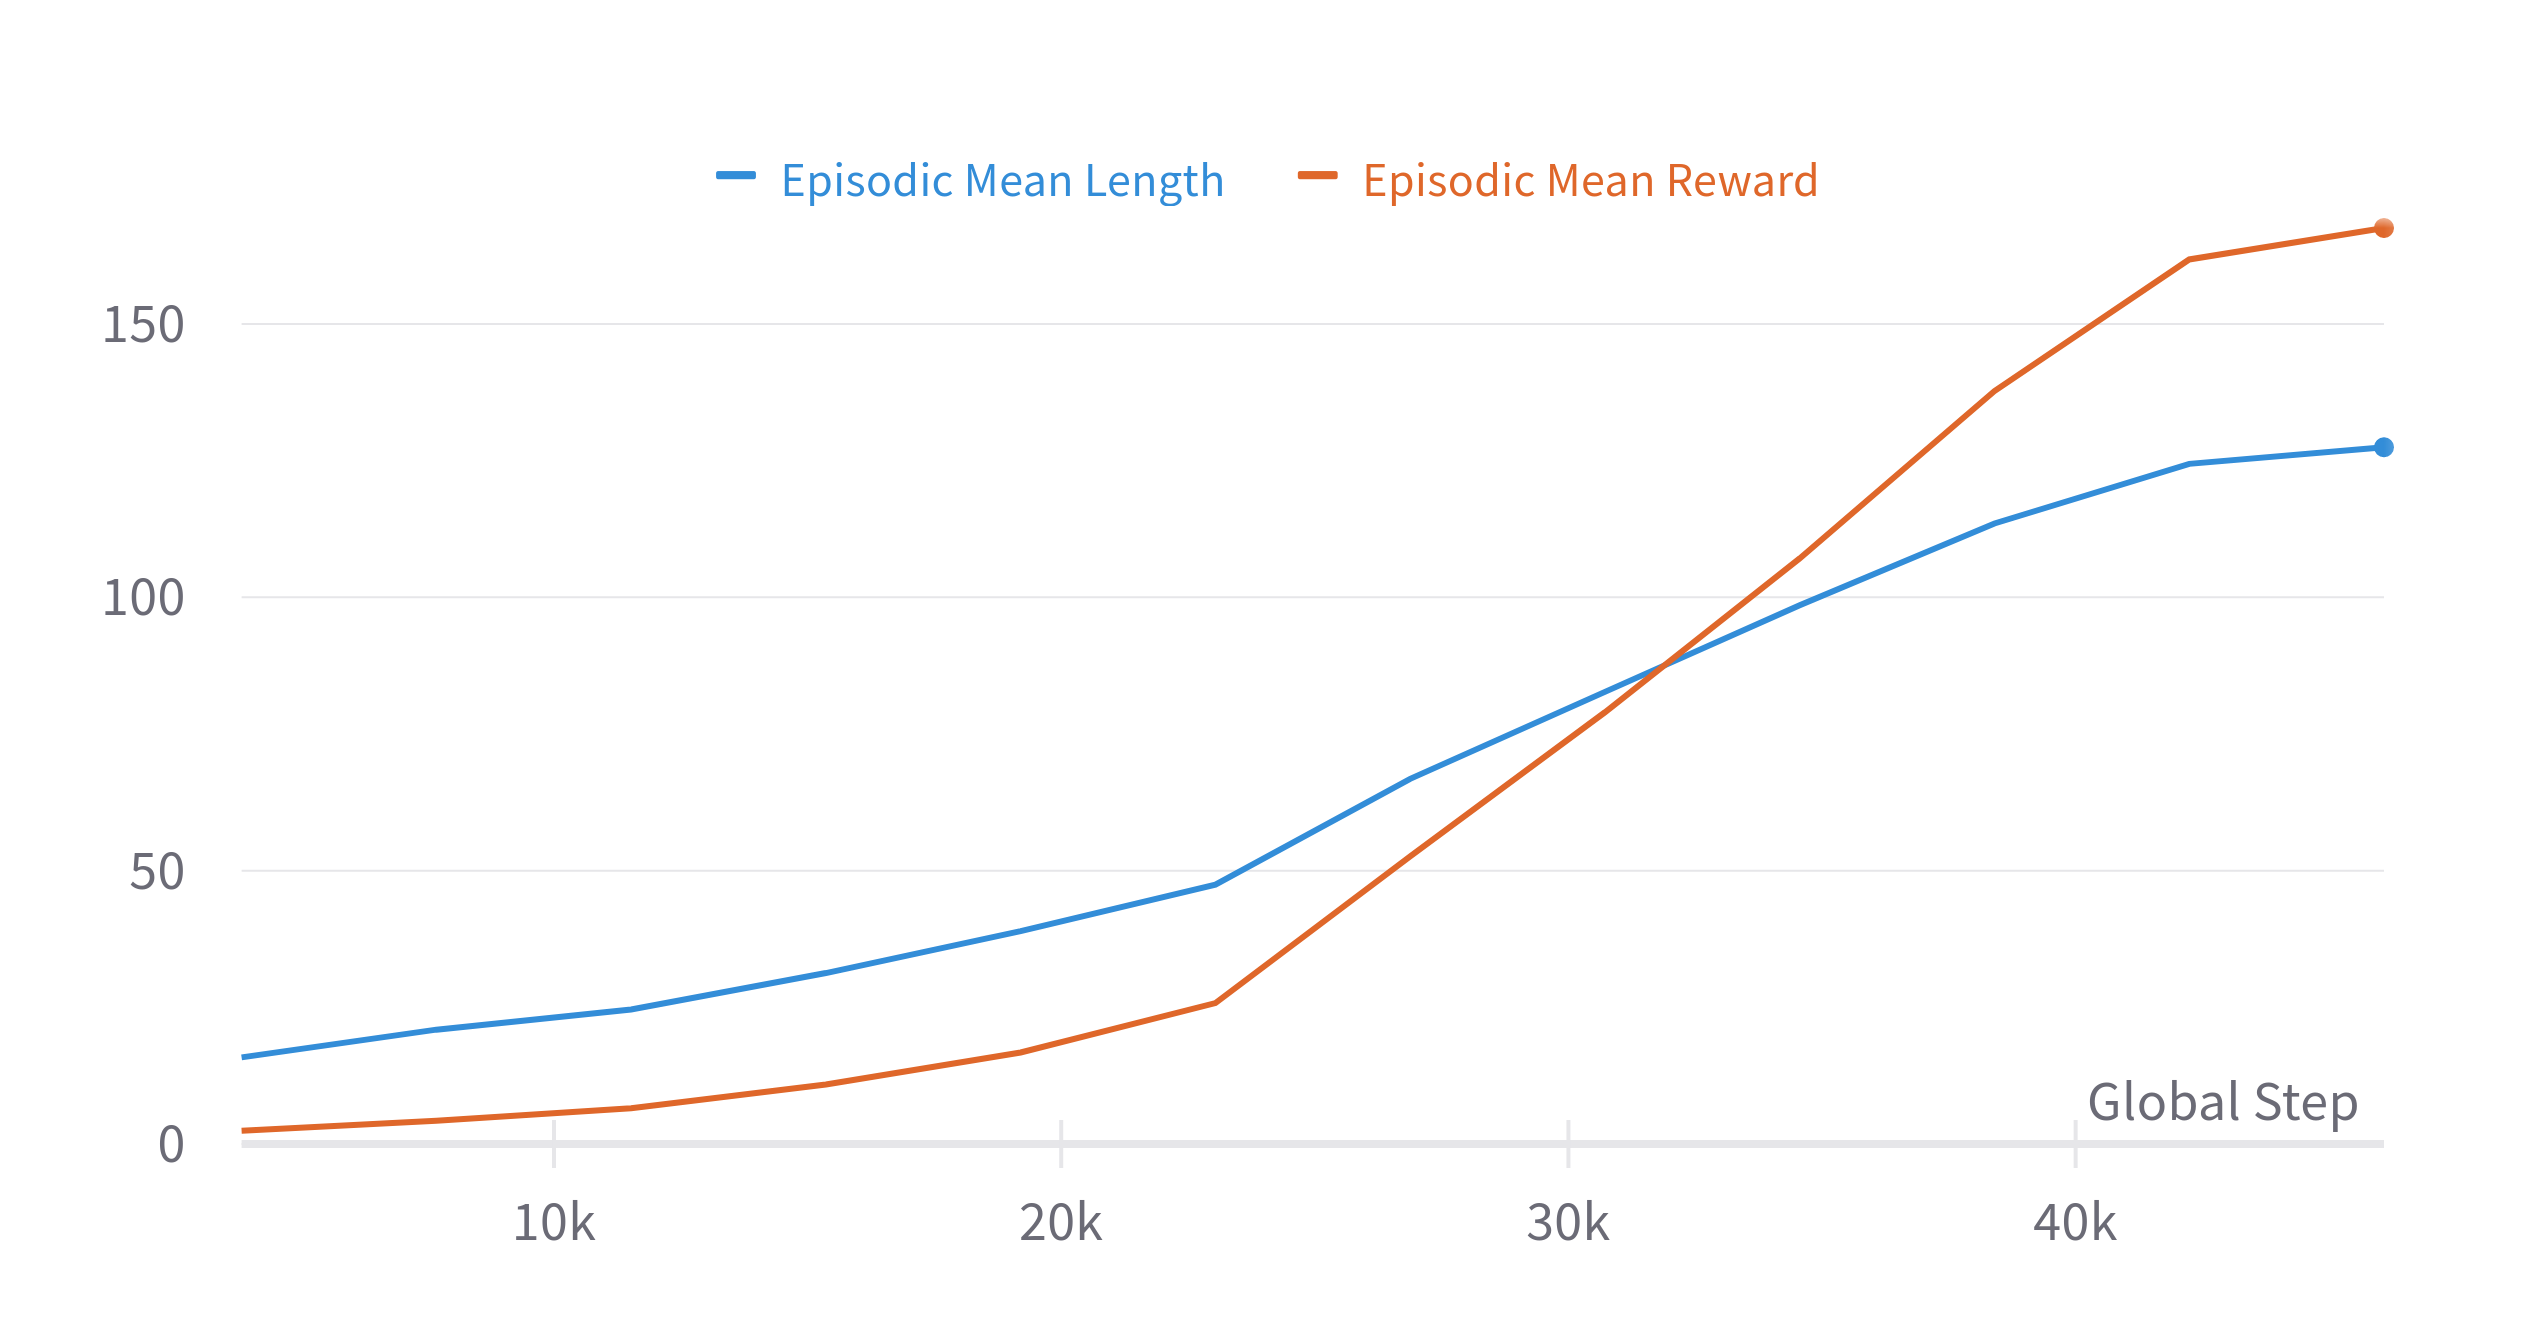
\includegraphics[width=0.45\textwidth]{Images/Results/rollout_cartpole.png}}
\end{figure}

As expected, the explained variance gets closer to $1$ as the training progresses, while the approximated KL divergence remains small, which means that the policy update is not too large. The value loss decreases as the training progresses, which means that the value function is getting better at predicting the return. The rollout metrics show that the mean reward and the mean episode length increase as the training progresses, which means that the policy is getting better at solving the task.

\subsubsection{Stickbot Locomotion}

In \cref{fig:stickbotresults}, the metrics obtained during the training with \textsc{Isaac gym} are reported.

\begin{figure}[h]
    \centering
    \caption{Stickbot RL Training Metrics}
    \label{fig:stickbotresults}
    \subfloat[Episodic Mean Length]{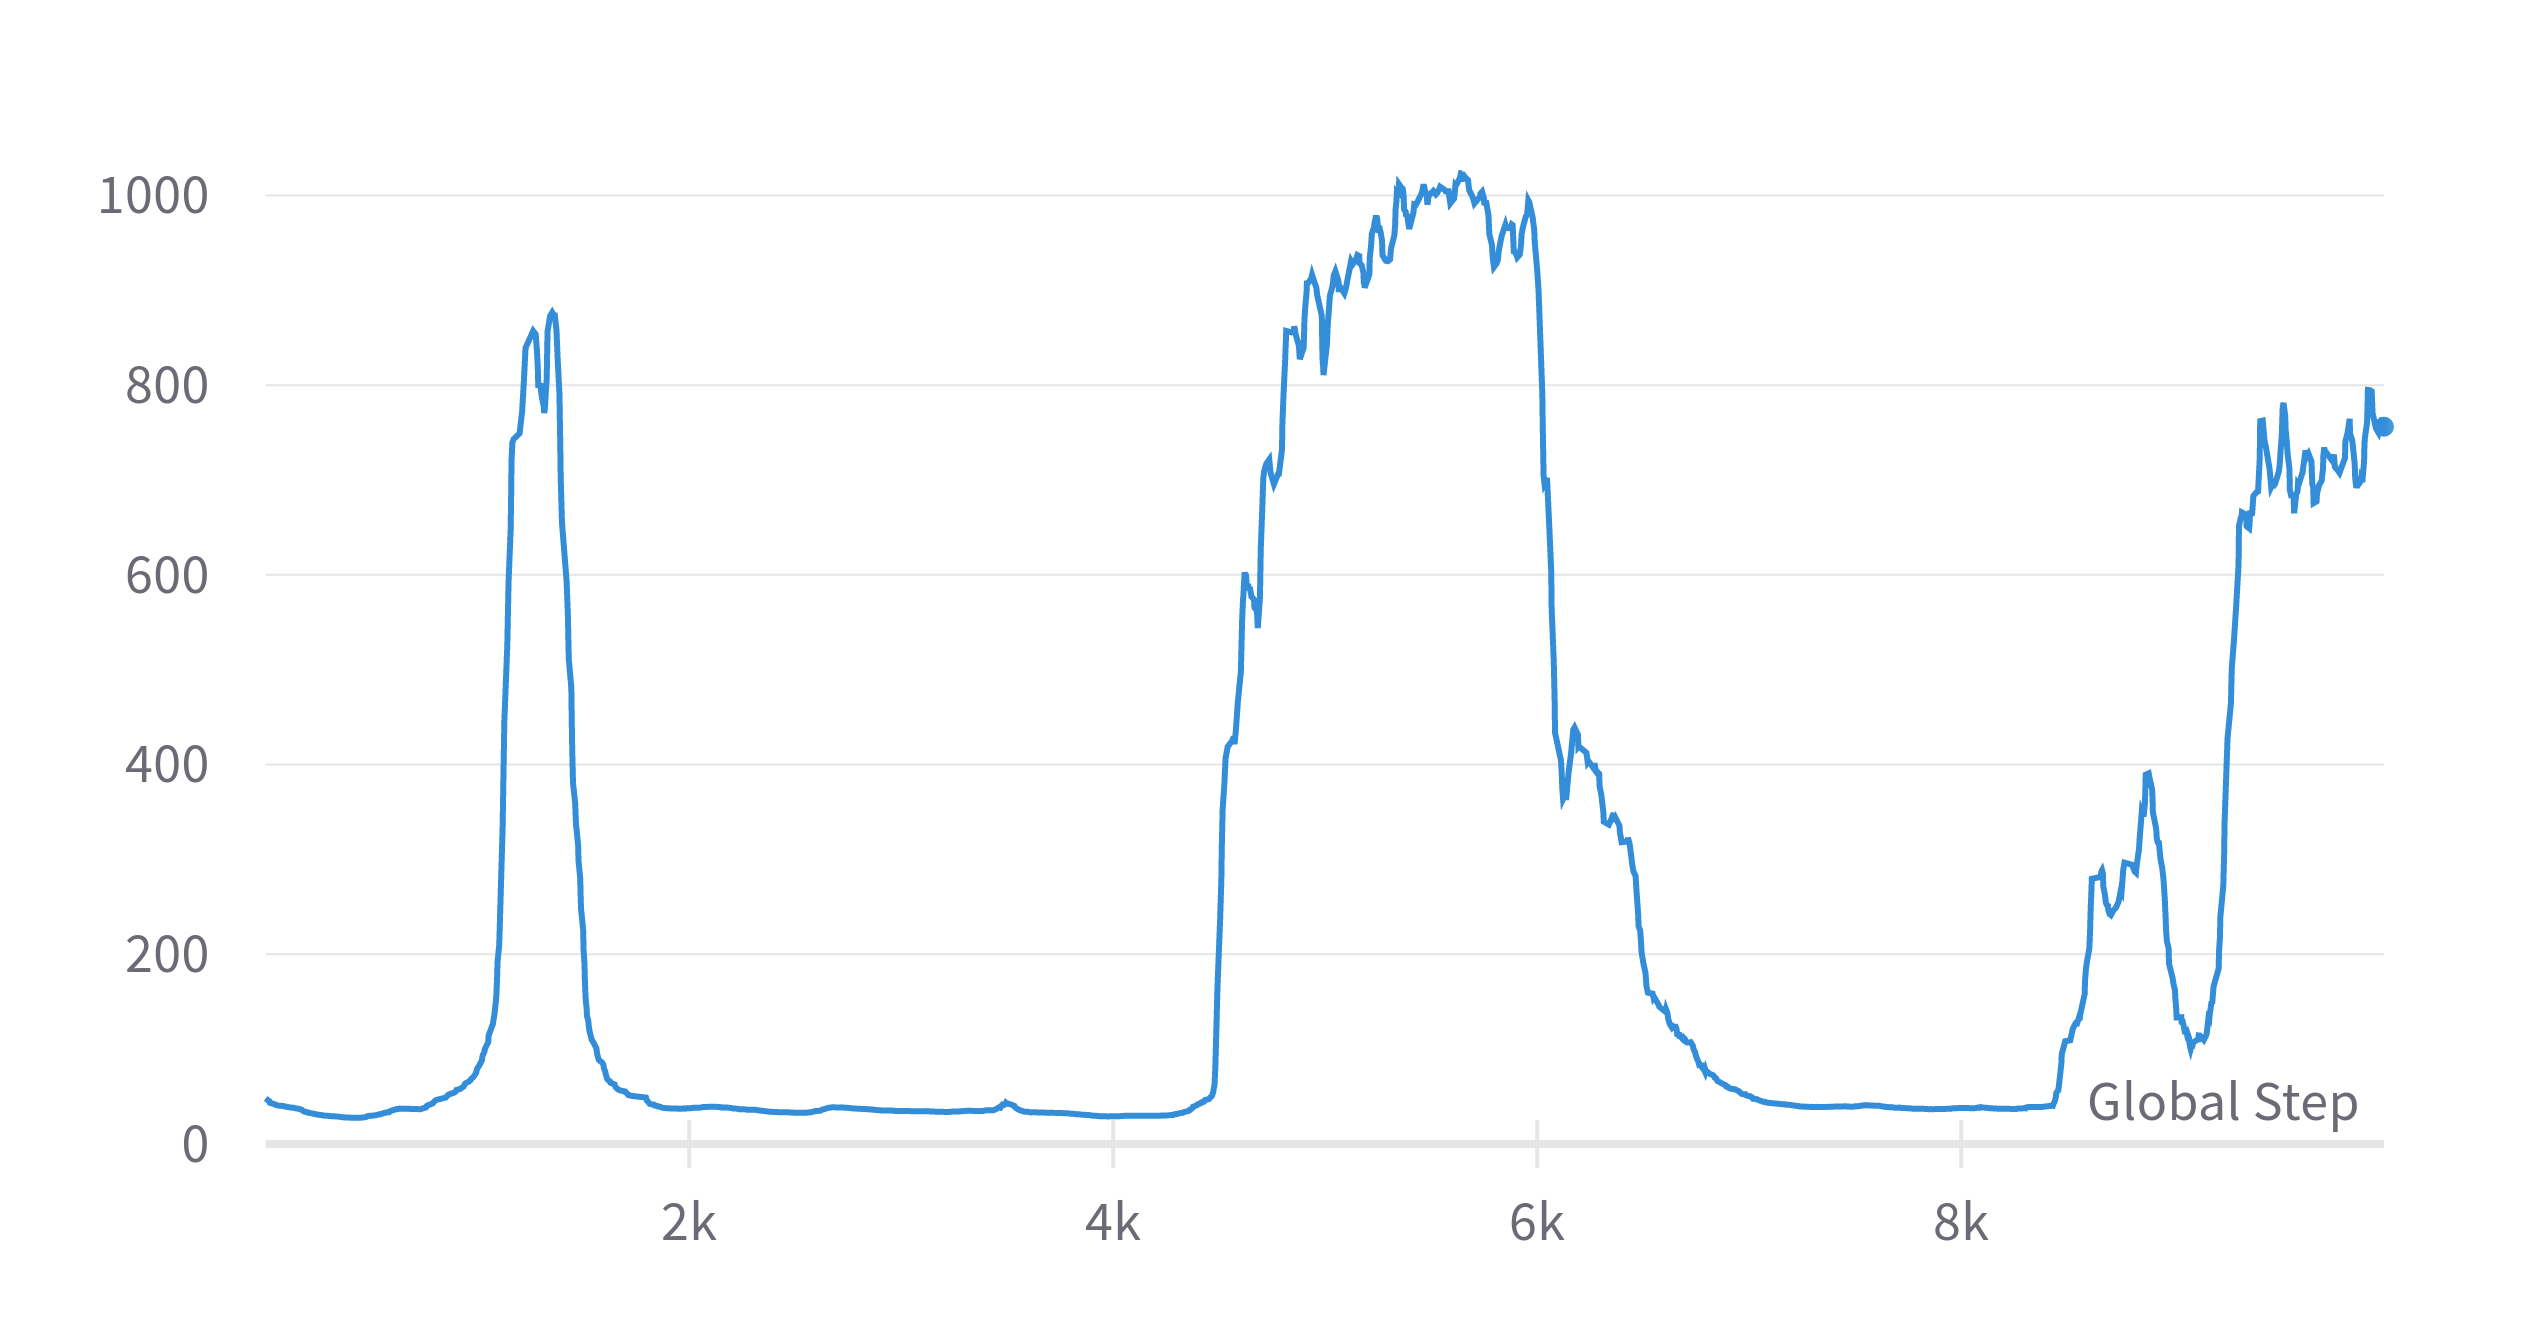
\includegraphics[width=0.45\textwidth]{Images/Results/rollout_eplen_stickbot.png}}
    \subfloat[Episodic Mean Reward]{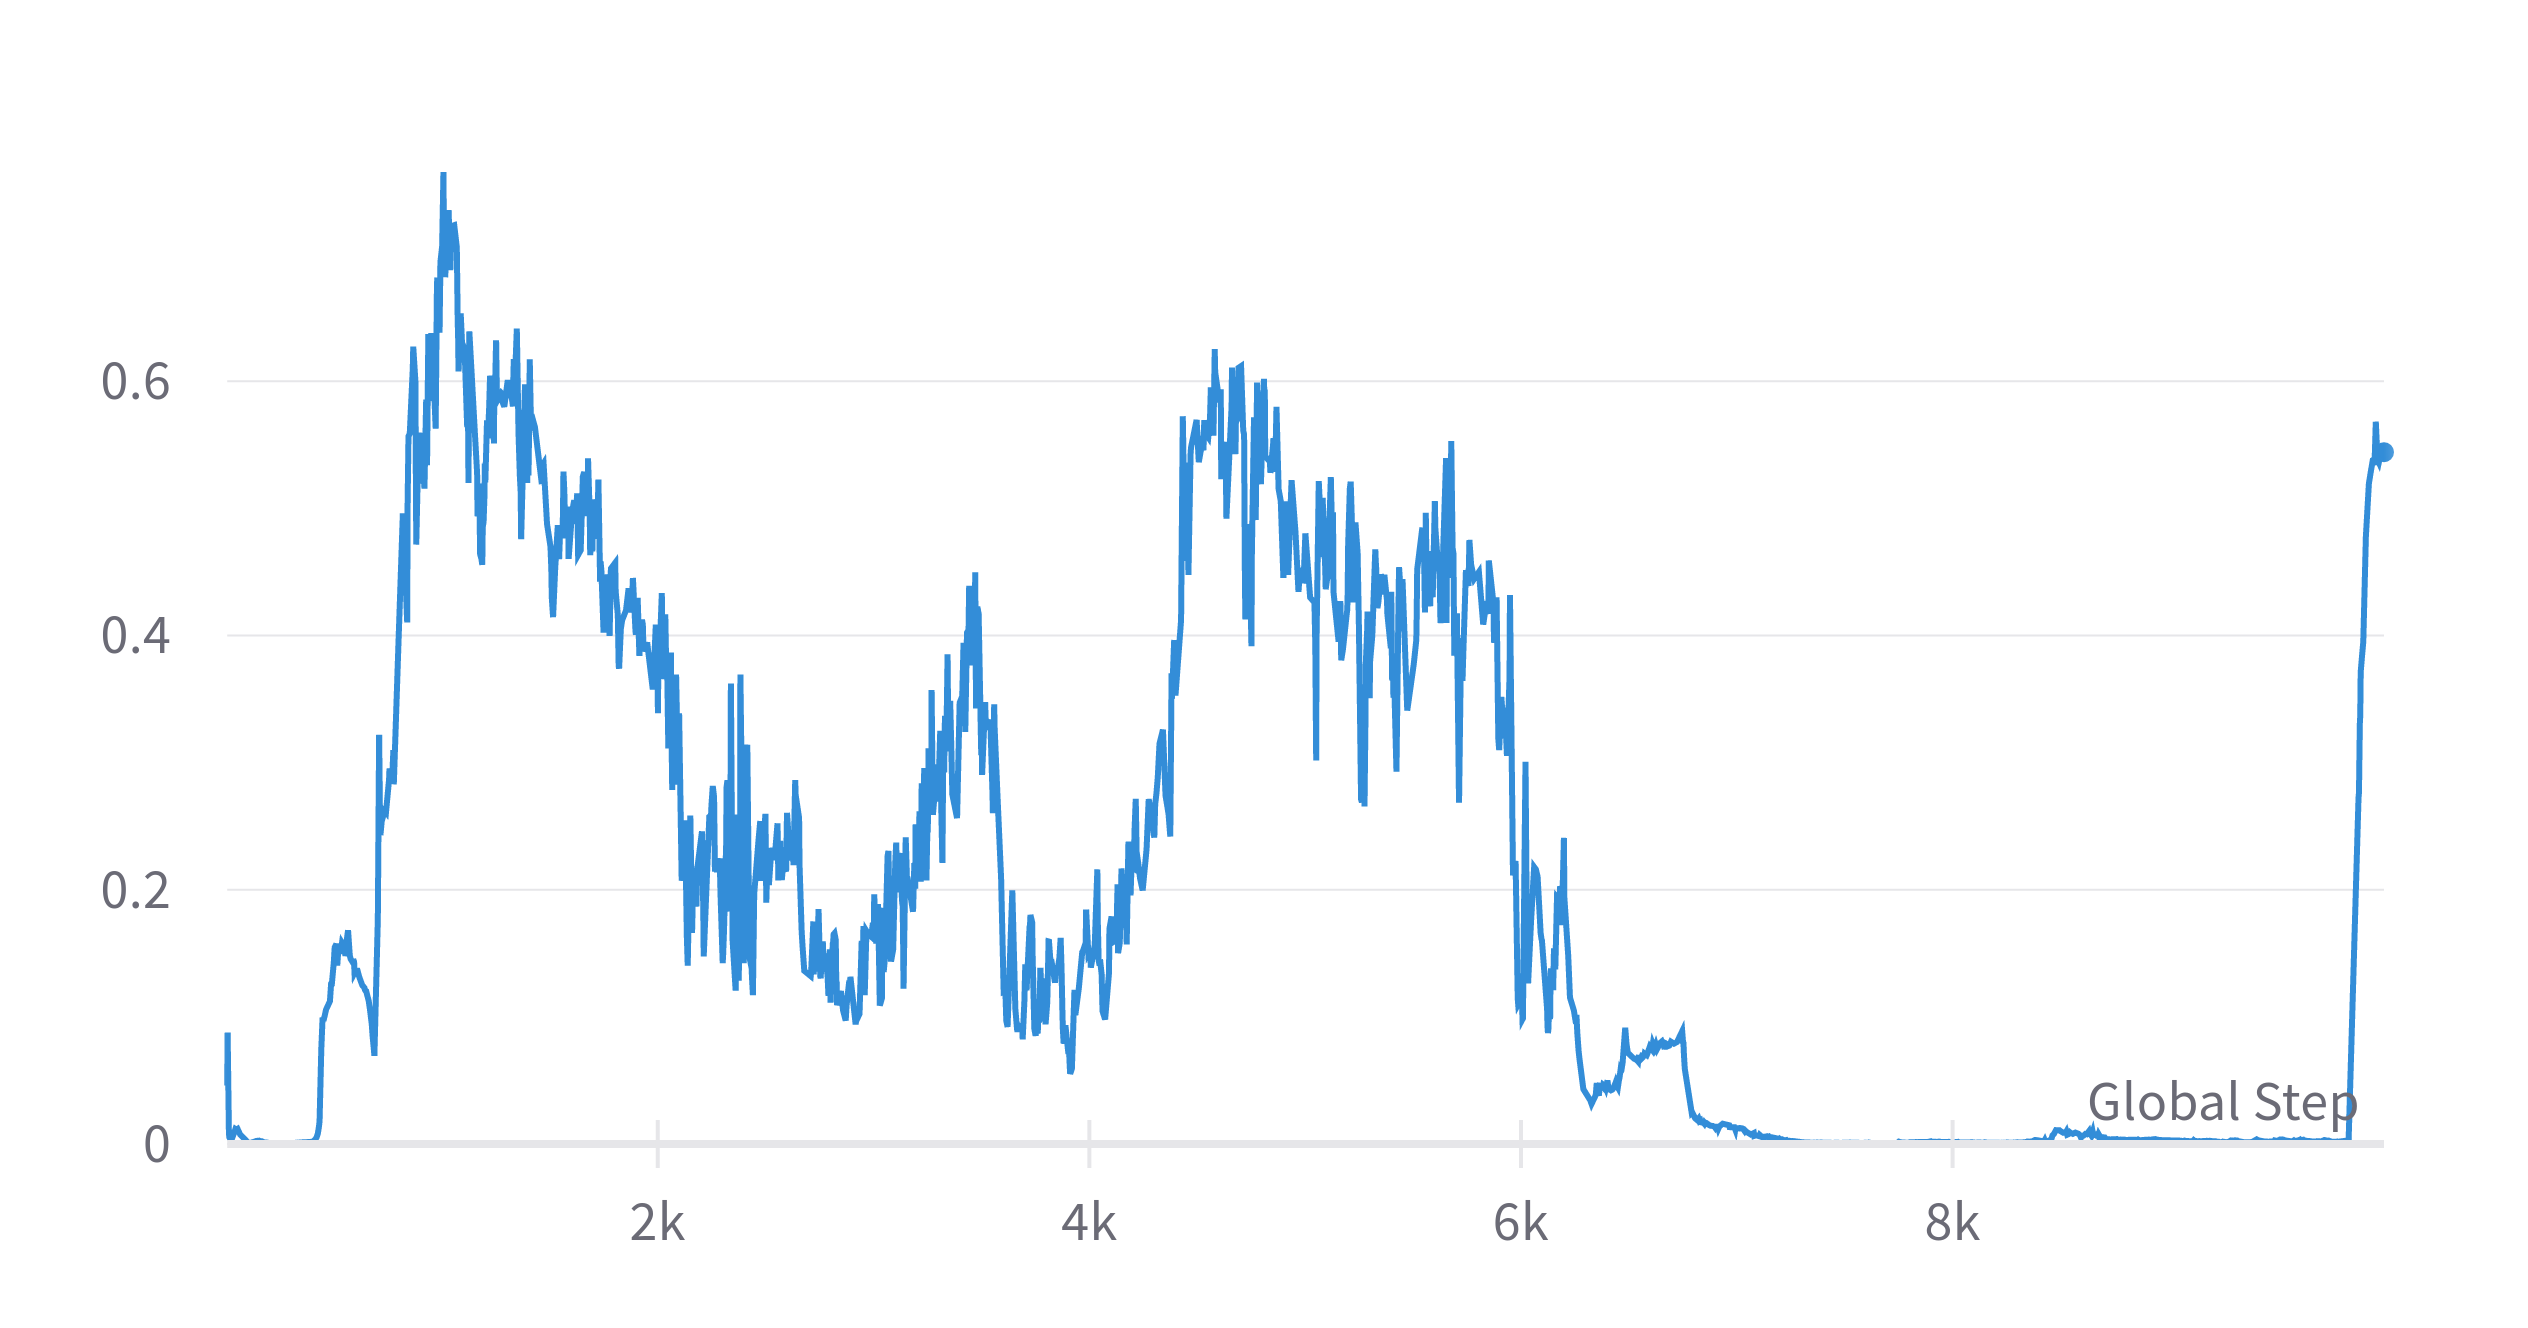
\includegraphics[width=0.45\textwidth]{Images/Results/rollout_meanrew_stickbot.png}}
\end{figure}

The mean episode length and the mean reward increase as the training progresses, which means that the policy is effectively learning to solve the task maximizing the reward.

\subsection{Codesign with Genetic Algorithm}

\begin{figure}[h]
    \centering
    \caption{Cartpole Codesign Results}
    \subfloat[Fitness Plot \label{fig:fitness}]{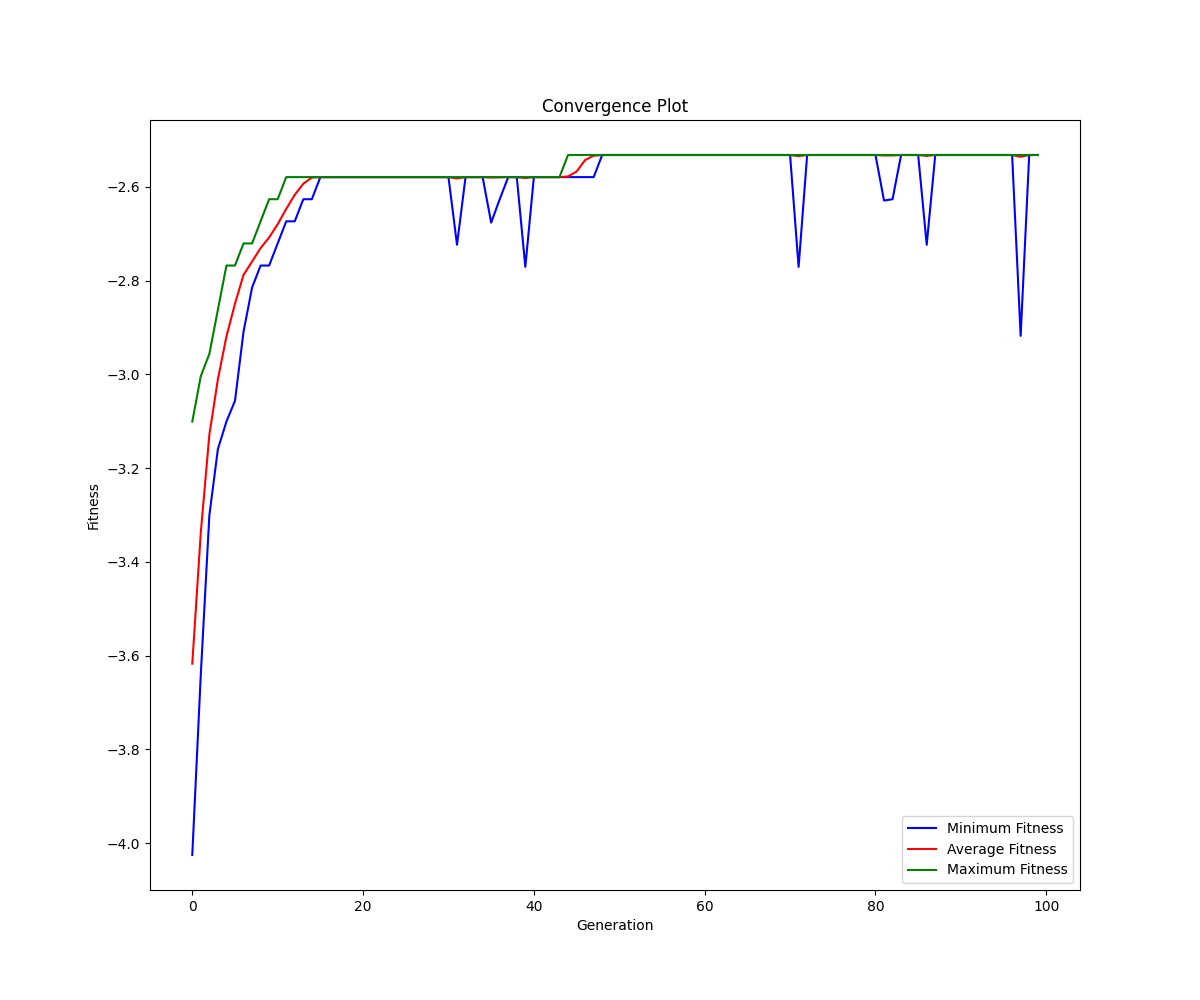
\includegraphics[width=0.4\textwidth]{Images/fitness.png}}
    \subfloat[Diversity Plot \label{fig:diversity}]{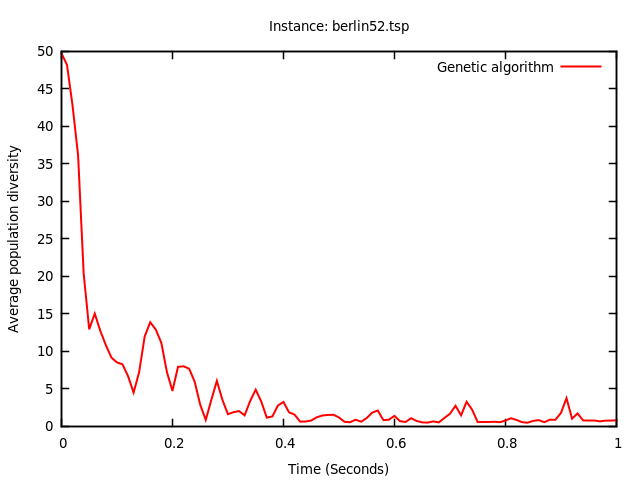
\includegraphics[width=0.4\textwidth]{Images/diversity.png}}
\end{figure}

In this section, we present the results obtained with the genetic algorithm. In particular, we present the results obtained with the codesign
framework for the \textit{Cartpole}.

As we can see from \cref{fig:fitness}, the convergence is achieved after SOME generations, with a fitness value of SOME. The diversity decreases as expected, as the population converges to the optimal solution, as we can see from \cref{fig:diversity}.